\chapter{Derivative of the Contrast Metric}\label{sec:jacobian}
Since we use bilinear voting to evaluate the \textit{dirac delta}, the
derivatives of the cost function \cref{eq:variance} can be
analytically computed as
\begin{align}
  \intertext{Let}
  \rho\left(\vec{x};\bm{\theta}\right)&=\mathcal{I}\left(\vec{x};\bm{\theta}\right)-\mu\left(\mathcal{I}\left(\vec{x};\bm{\theta}\right)\right)\\
  \intertext{with}
  \mu\left(\mathcal{I}\left(\vec{x};\bm{\theta}\right)\right)&=\frac{1}{\mid\Omega\mid}\int_{\Omega}\mathcal{I}\left(\vec{x};\bm{\theta}\right)d\vec{x},\label{eq:mean}
                                                        \intertext{then}
                                                        \frac{\partial}{\partial\bm{\theta}}\mathrm{Var}\left(\mathcal{I}\left(\vec{x};\bm{\theta}\right)\right)&=\frac{2}{\mid\Omega\mid}\int_{\Omega}\rho\left(\vec{x};\bm{\theta}\right)\frac{\partial\rho\left(\vec{x};\bm{\theta}\right)}{\partial{\bm{\theta}}}d\vec{x}    \label{eq:dVdw}
\end{align}
The derivatives of the warped image are
\begin{equation}
  \label{eq:dIdw}
  \frac{\partial\mathcal{I}\left(\vec{x};\bm{\theta}\right)}{\partial{\bm{\theta}}}=-\sum_{k=1}^N\pm_k\nabla\delta\left(\vec{x}-\vec{x}'_k\left(\bm{\theta}\right)\right)\frac{\partial\vec{x}'_k\left(\bm{\theta}\right)}{\partial\bm{\theta}},
\end{equation}
In the case of planar homography the events warping is computed as
\begin{align}
  \bm{\theta}&=\left(\bm{\omega}^\top,\vec{v}^\top,\varphi,\psi\right)^\top\in\mathbb{R}^8\\
  \vec{x}'_k\left(\bm{\theta}\right)&=
                                      \begin{bmatrix}
                                        x'_{im}&y'_{im}
                                      \end{bmatrix}^\top=
                                                 \begin{bmatrix}
                                                   x'/z'&y'/z'
                                                 \end{bmatrix}^\top\\
  \bar{\vec{x}}'_k\left(\bm{\theta}\right)&=
                                            \begin{bmatrix}
                                              x'&y'&z'
                                            \end{bmatrix}^\top\nonumber\\&=
  \mat{P}\left(\mat{R}_t^\top\left(\mat{I}+\vec{t}_t\vec{n}^\top/d\right)\right)^{-1}\bar{\vec{x}}_k\nonumber\\
             &=
               \mat{P}\left(\mat{I}+\vec{v}t\vec{n}^\top\right)^{-1}\mat{R}_t
               \bar{\vec{x}}_k, \label{eq:x_x}
               % &=
               % \mat{P}\left(\mat{I}-\frac{\vec{v}t\vec{n}^\top}{\vec{n}^\top\vec{v}t+1}\right)\mathrm{exp}(\bm{\omega}^\wedge
               % t)\vec{x}_k,
\end{align}
where $\mat{P}$ is the projection matrix from the camera frame to the
world frame or the map, which does not have to correspond with the
camera matrix provided by the data set. Also, for simplicity of
notation we assume $d = 1$, and denote
$\mat{P}\left(\mat{I}+\vec{v}t\vec{n}^\top\right)^{-1}$ as
$\mat{P_v}$. Since $t$ usually spans a small temporal window, we can
simplify the derivative with respect to angular velocity as
\begin{align}
  \mat{R}_t& =\mathrm{exp}(\bm{\omega}^\wedge t)\approx\mat{I}+\bm{\omega}^\wedge t\\
  \frac{\partial\bar{\vec{x}}'_k}{\partial\bm{\omega}}&=-\mat{P_v}t\bar{\vec{x}}_k^\wedge.  \label{eq:dxdo}
\end{align}
The above equation makes use of the equivalence
$\bm{\omega}\times\bar{\vec{x}}_k=-\bar{\vec{x}}_k\times\bm{\omega}$.

The derivative with respect to the linear velocity is
\begin{equation}
  \frac{\partial\bar{\vec{x}}'_k}{\partial\vec{v}}=-\frac{t\vec{n}^\top\mat{R}_t\vec{x}_k}{\vec{n}^\top\vec{v}t+1}\mat{P_v} \label{eq:dxdv}
\end{equation}
Similarly we have
\begin{align}
  \frac{\partial\bar{\vec{x}}'_k}{\partial\vec{n}}&=-\frac{t\vec{v}^\top\mat{R}_t\vec{x}_k}{\vec{n}^\top\vec{v}t+1}\mat{P_v} \\
  \intertext{and}
  \frac{\partial\bar{\vec{x}}'_k}{\partial(\varphi;\psi)}&= \frac{\partial\bar{\vec{x}}'_k}{\partial\vec{n}}\frac{\partial\vec{n}}{\partial(\varphi;\psi)},\\
  \intertext{with}
  \frac{\partial\vec{n}}{\partial(\varphi;\psi)}&=
                                                  \begin{bmatrix}
                                                    -\sin\varphi\sin\psi&\cos\varphi\cos\psi\\
                                                    \cos\varphi\sin\psi&\sin\varphi\cos\psi\\
                                                    0&-\sin\psi
                                                  \end{bmatrix}
                                                       \label{eq:dvdn}
\end{align}
With the above quantities
\begin{equation*}
  \label{eq:dx_dtheta}
  \frac{\partial\bar{\vec{x}}'_k}{\partial\bm{\theta}}=
  \begin{bmatrix}
    \frac{\partial\bar{\vec{x}}'_k}{\partial\bm{\omega}}&
    \frac{\partial\bar{\vec{x}}'_k}{\partial\vec{v}}&
    \frac{\partial\bar{\vec{x}}'_k}{\partial\varphi}&\frac{\partial\bar{\vec{x}}'_k}{\partial\psi}
  \end{bmatrix}\in\mathbb{R}^{3\times8}
\end{equation*}
we can compute the gradient
$\frac{\partial\vec{x}'_k}{\partial\bm{\theta}}$ as
\begin{equation}
  \label{eq:dxdtheta}
  \frac{\partial\vec{x}'_k}{\partial\bm{\theta}}=\left[\frac{\partial\bar{\vec{x}}'_k}{\partial\bm{\theta}}\frac{1}{z'}-\bar{\vec{x}}'_k\frac{\partial z'}{\partial\bm{\theta}}\frac{1}{z'^2}\right]_{1:2},
\end{equation}
and the third component of the derivative within the bracket is equal
to zero.

Theoretically, to evaluate the derivative of the cost function, the
dirac delta $\nabla\delta(\vec{x})$ should be evaluated at each pixel
location ($240\times180$ for DAVIS). However, since we are using
bilinear voting, a infinitesimal change $d\vec{x}$ at an event
location $\vec{x}$ will only affect the derivative evaluated at the
four neighboring pixels of $\vec{x}$. An illustration is shown in
\cref{fig:bi_voting}

\begin{figure}
  \begin{minipage}[t]{0.48\textwidth}
    \centering 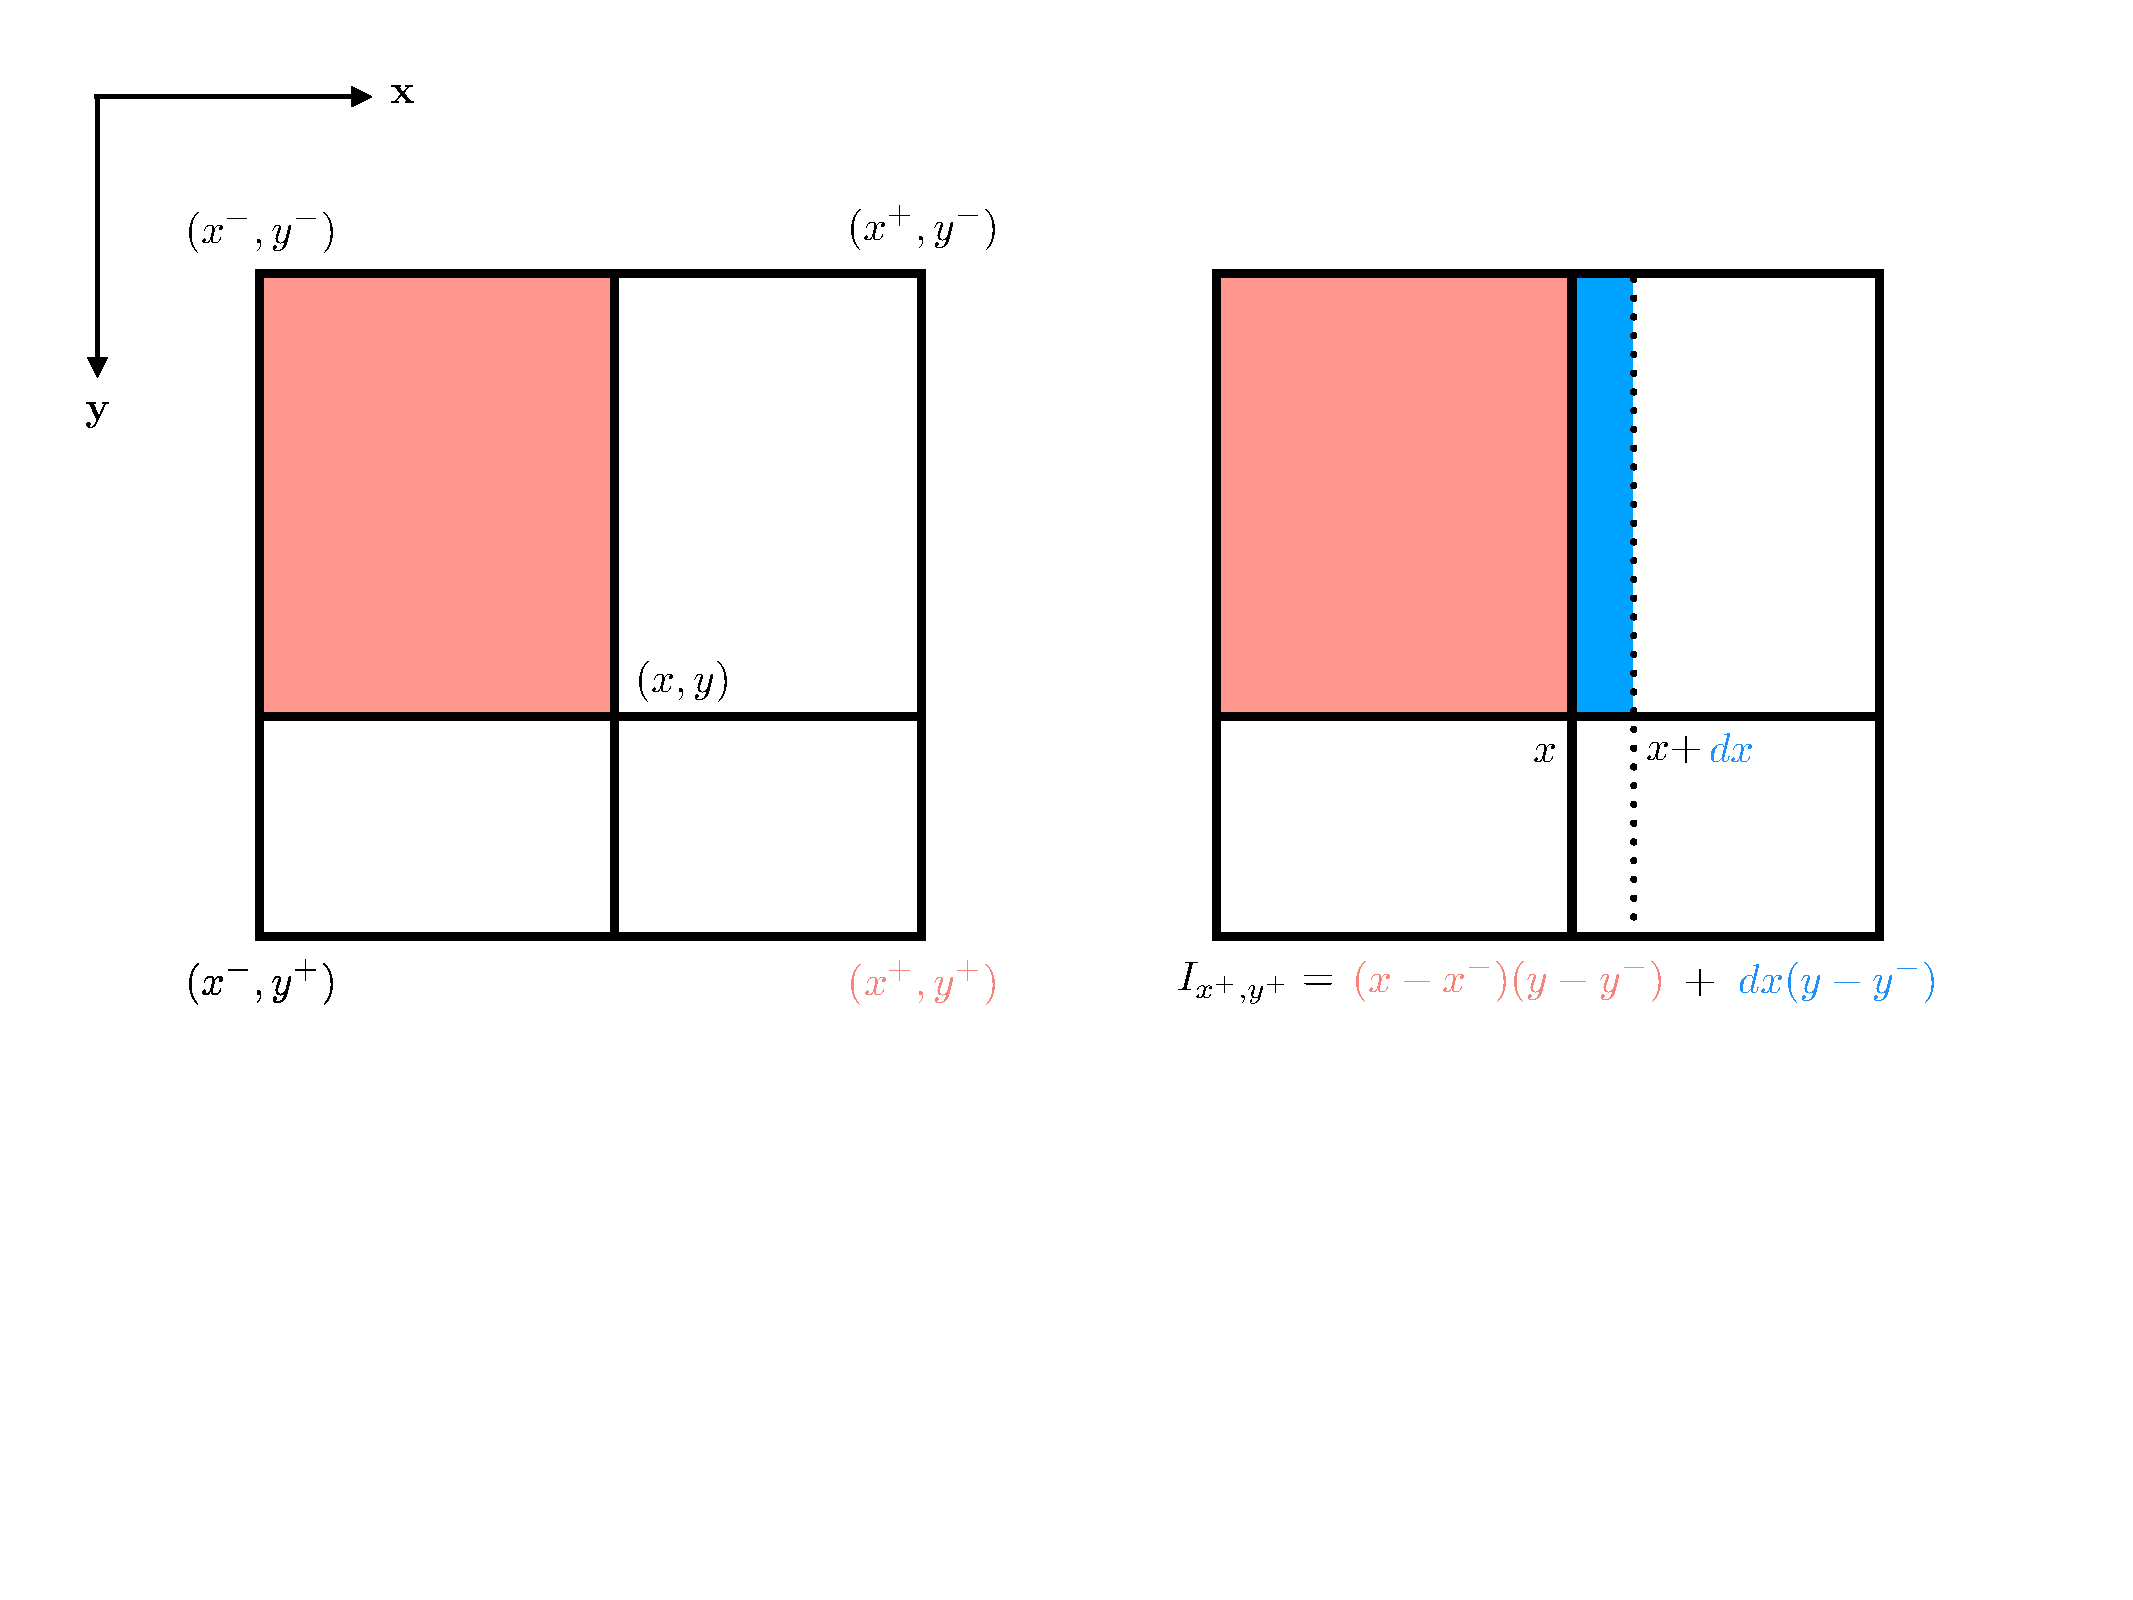
\includegraphics[trim={1cm 7cm 18cm 1cm},clip,width =
    \textwidth]{images/bi_voting.pdf} (a) The intensity at a pixel
    location is the area of the rectangle spanned by the opposite
    pixel and the event location
  \end{minipage}
  \hfill
  \begin{minipage}[t]{0.48\textwidth}
    \centering 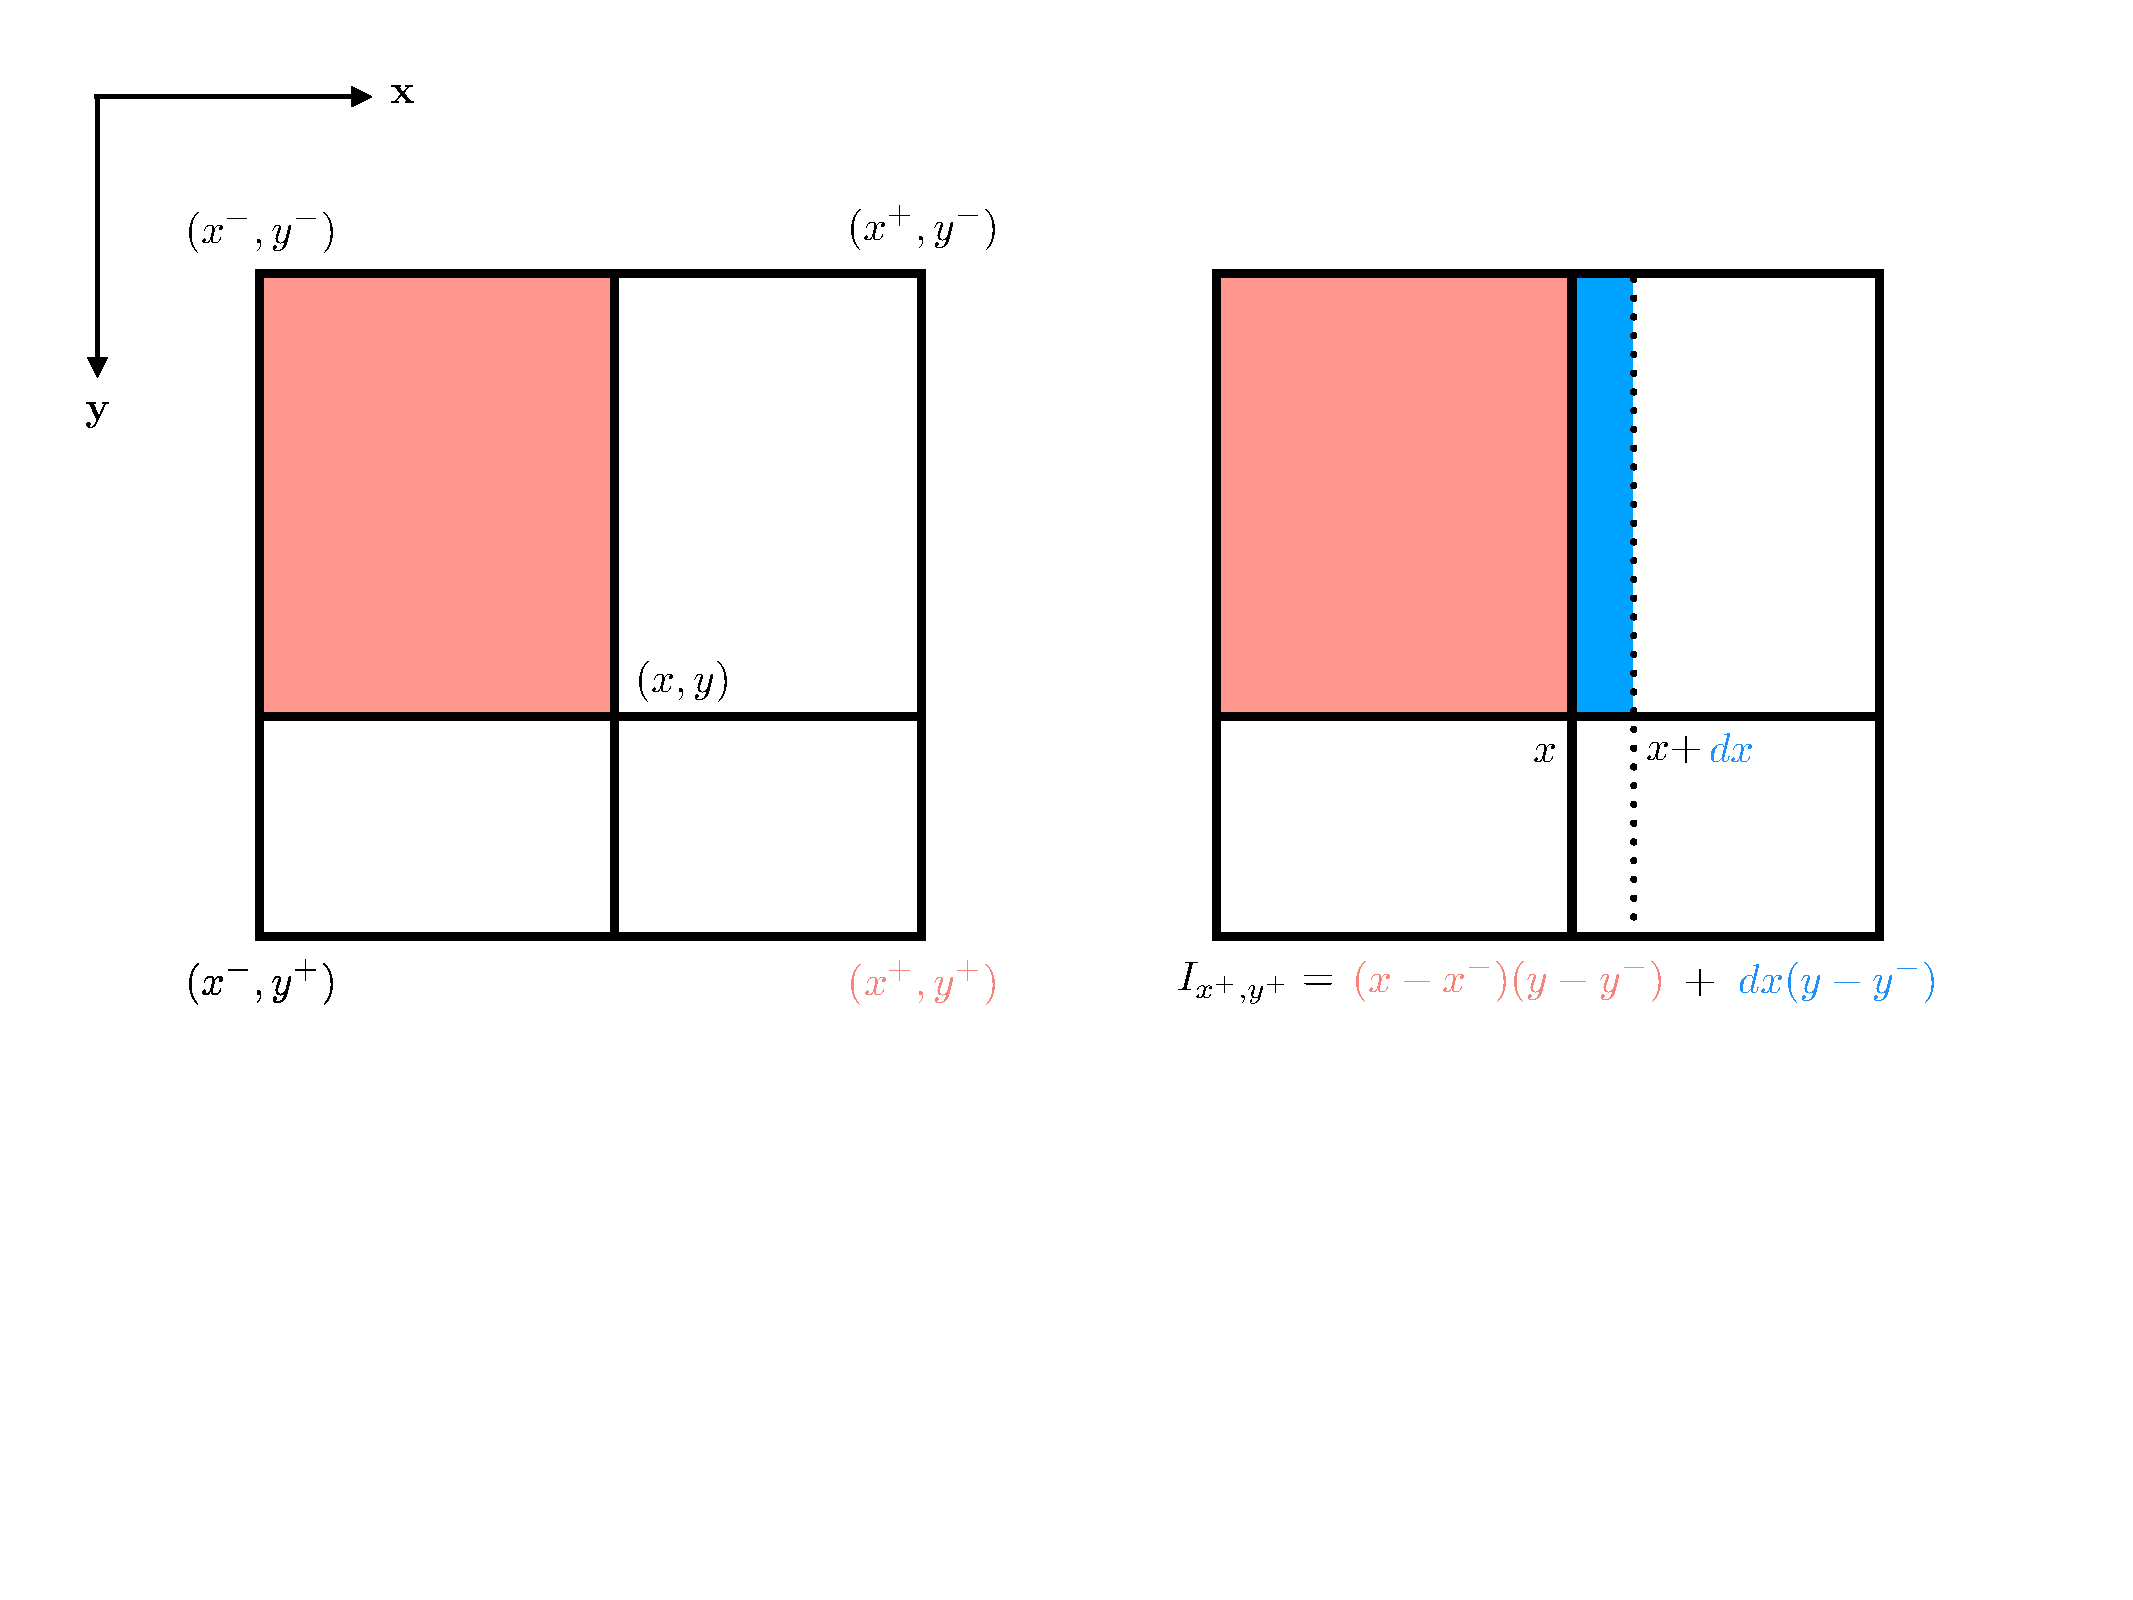
\includegraphics[trim={18cm 7cm 1cm 1cm},clip,width =
    \textwidth]{images/bi_voting.pdf} (b) Intensity change after an
    infinitesimal movement of the event
  \end{minipage}
  \caption{Bilear voting}
  \label{fig:bi_voting}
\end{figure}
The detailed algorithm for the evaluation of the Dirac delta as well
as its derivative is shown in algorithm.~\ref{alg:bi_voting}. The
behavior of the bilinear voting for derivatives is undefined when
$\vec{x}_k'$ locates exactly at a pixel location. However, the
possibility of this to happen is zero except when $t=0$, and can be
solved by simply discarding the event or disturbing with a small
random noise. When projecting back to the map, The author uses a
project matrix with different focal lengths than the ones in the
camera calibration matrix, so that there won't be event at integer
pixel locations after warping.
\begin{algorithm}
  \DontPrintSemicolon \SetAlgoLined \SetKwInOut{Input}{Input}
  \SetKwInOut{Output}{Output} \Input{A warped event
    $e'_k=\{x_k',y_k',t_k\}$} \Output{The \textit{Dirac delta}
    $\delta(\vec{x}-\vec{x}'_k)$ as well as its derivative
    $\frac{\partial\delta(\vec{x}-\vec{x}'_k)}{\partial\vec{x}'_k}$}
  \hrule\; Let\;
  $x^-=\lfloor x'_k\rfloor, x^+=\lceil x'_k\rceil,y^-=\lfloor
  y'_k\rfloor, y^+=\lceil y'_k\rceil$\; Then\;
  $\delta(x^--x'_k,y^--y'_k)=(x-x^+)(y-y^+)$\;
  $\delta(x^--x'_k,y^+-y'_k)=-(x-x^+)(y-y^-)$\;
  $\delta(x^+-x'_k,y^--y'_k)=-(x-x^-)(y-y^+)$\;
  $\delta(x^+-x'_k,y^+-y'_k)=(x-x^-)(y-y^-)$\;
  $\frac{\partial\delta(x^--x'_k,y^--y'_k)}{\partial
    x'_k}=y-y^+,\frac{\partial\delta(x^--x'_k,y^--y'_k)}{\partial
    y'_k}=x-x^+$\;
  $\frac{\partial\delta(x^--x'_k,y^+-y'_k)}{\partial
    x'_k}=-(y-y^-),\frac{\partial\delta(x^--x'_k,y^+-y'_k)}{\partial
    y'_k}=-(x-x^+)$\;
  $\frac{\partial\delta(x^+-x'_k,y^--y'_k)}{\partial
    x'_k}=-(y-y^+),\frac{\partial\delta(x^+-x'_k,y^--y'_k)}{\partial
    y'_k}=-(x-x^-)$\;
  $\frac{\partial\delta(x^+-x'_k,y^+-y'_k)}{\partial
    x'_k}=y-y^-,\frac{\partial\delta(x^+-x'_k,y^+-y'_k)}{\partial
    y'_k}=x-x^-$\;
  \caption{Bilinear Voting}
  \label{alg:bi_voting}
\end{algorithm}
\BlankLine For better convergence behavior, we smooth
$\mathcal{I}\left(\vec{x};\bm{\theta}\right)$ by a Gaussian with a
sigma of 1 as in\citep{gallego2017accurate}. Although for each event
the jacobian only considers the four neighbors, the smoothing
operation spreads this to broader pixels, leading to a smoother cost
function which is easier to optimize.
